\documentclass[12pt,utf8,notheorems,compress]{beamer}
\usepackage{etex}

\usepackage[ngerman]{babel}

\usepackage{amsmath,amssymb}
%\usepackage[framed,amsmath,thmmarks,hyperref]{ntheorem}

%\usepackage[small,nohug]{diagrams}
%\diagramstyle[labelstyle=\scriptstyle]

%\usepackage[protrusion=true,expansion=false]{microtype}

%\usepackage{lmodern}
\usepackage{tabto}
\usepackage{tikz}
\usepackage{array}
\usepackage[all]{xy}

%\usepackage[natbib=true,style=numeric]{biblatex}
%\usepackage[babel]{csquotes}
%\bibliography{lit}

%\usepackage{hyperref}

\setlength\parskip{\medskipamount}
\setlength\parindent{0pt}

%\theoremseparator{:}
\theoremstyle{plain}  %nonumberplain
%\newtheorem{beh}{Behauptung}
\newtheorem{proposition}{Proposition}
\newtheorem{corollary}{Korollar}
\newtheorem{theorem}{Satz}
\theoremstyle{definition}
\newtheorem{definition}{Definition}
%\newtheorem{kor}{Korollar}
%\newtheorem{satz}{Satz}
%\newtheorem{lemma}{Lemma}
%\newtheorem{hilfsaussage}{Hilfsaussage}
%\theorembodyfont{\normalfont}
\newtheorem{axiom}{Axiom}
%\newtheorem{defnprop}{Definition/Proposition}
%\newtheorem{bem}{Bemerkung}
%\newtheorem{bsp}{Beispiel}
%\theoremsymbol{\ensuremath{\openbox}}
%\newtheorem{proof}{Beweis}
%\newtheorem{defn}{Definition}

\newcommand{\lra}{\longrightarrow}
\newcommand{\lhra}{\ensuremath{\lhook\joinrel\relbar\joinrel\rightarrow}}
\newcommand{\thlra}{\relbar\joinrel\twoheadrightarrow}

\newcommand{\Z}{\mathbb{Z}}
\renewcommand{\C}{\mathcal{C}}
\newcommand{\N}{\mathbb{N}}
\newcommand{\R}{\mathbb{R}}
\newcommand{\Hom}{\mathrm{Hom}}
\newcommand{\id}{\mathrm{id}}
\newcommand{\Aut}[1]{\operatorname{Aut}(#1)}
\newcommand{\GL}[1]{\operatorname{GL}(#1)}
\newcommand{\freist}{\_{}\_{}}
\newcommand{\Set}{\mathrm{Set}}
\newcommand{\Grp}{\mathrm{Grp}}
\newcommand{\Vect}{\mathrm{Vect}}

\def\longleadsto{\mathrel{-}\joinrel\leadsto}
\DeclareMathOperator{\ggT}{ggT}
\DeclareMathOperator{\Ob}{Ob}
\newcommand{\op}{\mathrm{op}}

\title{Was sind und was sollen Kategorien?}
\author[Curry Club Augsburg]{%
  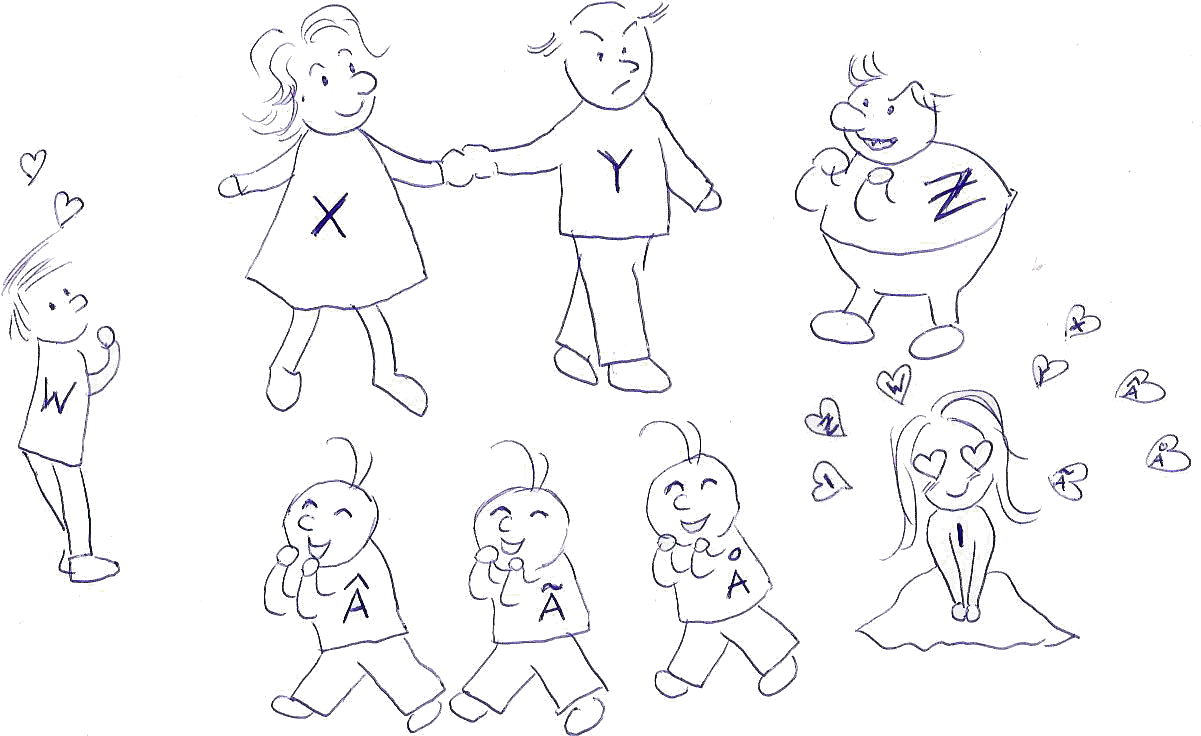
\includegraphics[scale=0.4]{relationen.png} \\\bigskip
  \footnotesize Ingo Blechschmidt}
\date{18. Juni 2015}

\usetheme{Warsaw}
\useoutertheme{split}
\usecolortheme{seahorse}
\usefonttheme{serif}
\usepackage{palatino}
\useinnertheme{rectangles}

\setbeamertemplate{navigation symbols}{}
%\setbeamertemplate{footline}{}
%\setbeamertemplate{headline}{}

\setbeamertemplate{title page}[default][colsep=-1bp,rounded=false,shadow=false,bg=white]
\setbeamertemplate{frametitle}[default][colsep=-2bp,rounded=false,shadow=false,center]
\setbeamertemplate{footline}{%
  \leavevmode%
  \hfill%
  \begin{beamercolorbox}[ht=2.25ex,dp=1ex,right]{}%
    \usebeamerfont{date in head/foot}
    \insertframenumber\,/\,\inserttotalframenumber\hspace*{1ex}
  \end{beamercolorbox}%
  \vskip0pt%
}


%\beamertemplateboldcenterframetitle
%\setbeamerfont{frametitle}{size={\Large}}

\newcommand*\oldmacro{}%
\let\oldmacro\insertshorttitle%
\renewcommand*\insertshorttitle{%
  \oldmacro\hfill\insertframenumber\,/\,\inserttotalframenumber\hfill}

\newenvironment{changemargin}[2]{%
  \begin{list}{}{%
    \setlength{\topsep}{0pt}%
    \setlength{\leftmargin}{#1}%
    \setlength{\rightmargin}{#2}%
    \setlength{\listparindent}{\parindent}%
    \setlength{\itemindent}{\parindent}%
    \setlength{\parsep}{\parskip}%
  }%
  \item[]}{\end{list}}

\newcommand{\slogan}[1]{%
  \begin{center}%
    \setlength{\fboxrule}{2pt}%
    \setlength{\fboxsep}{-3pt}%
    {\usebeamercolor[fg]{item}\fbox{\usebeamercolor[fg]{normal
    text}\parbox{0.9\textwidth}{\begin{center}#1\end{center}}}}%
  \end{center}%
}

\newcommand{\hil}[1]{{\usebeamercolor[fg]{item}{#1}}}

\begin{document}

\setbeameroption{hide notes}
\setbeamertemplate{note page}[plain]

\frame{\titlepage}
%\frame[t]{\frametitle{Gliederung}\begin{minipage}{\textwidth}\begin{small}\tableofcontents\end{small}\end{minipage}}
\frame[t]{\frametitle{Gliederung}\tableofcontents}

\section[Motivation]{Motivation: Beispiele für kategorielles Verständnis}

\subsection{Produkte}
\frame[t]{\frametitle{Produkte in Kategorien I}
  \begin{itemize}
    \item Kartesisches Produkt von Mengen: $X \times Y$
    \item Kartesisches Produkt von Vektorräumen: $V \times W$
    \item Kartesisches Produkt von Gruppen: $G \times H$
    \item Minimum von Zahlen: $\min\{n,m\}$
    \item Größter gemeinsamer Teiler von Zahlen: $\ggT(n,m)$
    \item Paartyp in Programmiersprachen: \texttt{(a,b)}
    \item Mutterknoten zweier Knoten in einem Graph
  \end{itemize}

  \slogan{%
    All dies sind Spezialfälle des allgemeinen \\ \emph{kategoriellen Produkts}.
  }

  \begin{tikzpicture}[remember picture,overlay]  
    \node [xshift=-1cm,yshift=-8.5cm] at (current page.north east)
      {
\includegraphics[scale=0.4]{produkt.png}};
  \end{tikzpicture}
}

\frame[t]{\frametitle{Produkte in Kategorien II}
  \begin{align*}
    X \times (Y \times Z) &\cong (X \times Y) \times Z \\
    U \times (V \times W) &\cong (U \times V) \times W \\
    \min\{m,\min\{n,p\}\} &= \min\{\min\{m,n\},p\} \\
    \ggT(m,\ggT(n,p)) &= \ggT(\ggT(m,n),p)
  \end{align*}

  \slogan{%
    All dies sind Spezialfälle der allgemeinen \\ \emph{Assoziativität} des kategoriellen Produkts.
  }

  \begin{tikzpicture}[remember picture,overlay]  
    \node [xshift=-1cm,yshift=-7.5cm] at (current page.north east)
      {
\includegraphics[scale=0.4]{produkt.png}};
  \end{tikzpicture}
}

\subsection{Isomorphismen}
\frame[t]{\frametitle{Isomorphismen in Kategorien}
  \begin{itemize}
    \item Zwei Mengen $X,Y$ \tabto{4.63cm} können gleichmächtig sein.
    \item Zwei Vektorräume $V,W$ \tabto{4.63cm} können isomorph sein.
    \item Zwei Gruppen $G,H$ \tabto{4.63cm} können isomorph sein.
    \item Zwei top. Räume $X,Y$ \tabto{4.63cm} können homöomorph sein.
    \item Zwei Zahlen $n,m$ \tabto{4.63cm} können gleich sein.
    \item Zwei Typen \texttt{a}, \texttt{b} \tabto{4.63cm} können sich verlustfrei ineinander umwandeln lassen.
  \end{itemize}

  \slogan{%
    All dies sind Spezialfälle des allgemeinen \\ \emph{kategoriellen
    Isomorphiekonzepts}.
  }

  \begin{tikzpicture}[remember picture,overlay]  
    \node [xshift=-1.1cm,yshift=-8.0cm] at (current page.north east)
      {
\includegraphics[scale=0.4]{isomorphie.png}};
  \end{tikzpicture}
}

\subsection{Dualität}
\frame[t]{\frametitle{Dualität}
  \vspace{-0.5em}
  \only<1>{
    \begin{center}
      \setlength{\extrarowheight}{0.3em}
      \begin{tabular}{r|l}
        $f \circ g$ & $g \circ f$ \\
        $\leq$ & $\geq$ \\
        injektiv & surjektiv \\
        $\{\star\}$ & $\emptyset$ \\
        $\times$ & $\amalg$ \\
        ggT & kgV \\
        $\cap$ & $\cup$ \\
        Teilmenge & Faktormenge
      \end{tabular}
    \end{center}
  }
  \only<2>{
    \begin{center}
      \setlength{\extrarowheight}{0.3em}
      \begin{tabular}{r|l}
        \texttt{(a,b)} & \texttt{Either a b} \\
        Typ der Streams & Typ der endlichen Listen \\
        Monaden & Komonaden \\
        Rechts-Kan-Erweiterung & Links-Kan-Erweiterung
      \end{tabular}
    \end{center}
  }

  \slogan{%
    All dies sind Spezialfälle eines allgemeinen \\
    \emph{kategoriellen Dualitätsprinzips}.
  }

  \begin{tikzpicture}[remember picture,overlay]  
    \node [xshift=-1cm,yshift=-7.5cm] at (current page.north east)
      {
\includegraphics[scale=0.4]{dualitaet.png}};
  \end{tikzpicture}
}


\section{Grundlagen}

\subsection[Def.]{Definition des Kategorienbegriffs}
\frame[t]{\frametitle{Kategorien}%
  \begin{tikzpicture}[remember picture,overlay]
    \node [xshift=-2cm,yshift=-2cm] at (current page.north east)
      {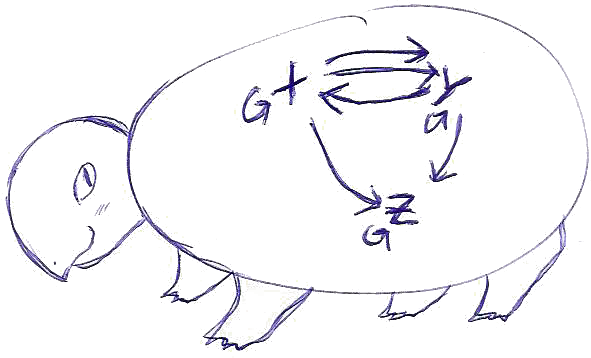
\includegraphics[scale=0.3]{kategorie.png}};
  \end{tikzpicture}%
  \small
  \textbf{Definition:} Eine Kategorie~$\C$ besteht aus
  \begin{enumerate}
    \item einer Klasse von \emph{Objekten} $\Ob \C$,
    \item zu je zwei Objekten $X,Y \in \Ob \C$ einer Klasse $\Hom_\C(X,Y)$ von
    \emph{Morphismen} zwischen ihnen und
    \item einer Kompositionsvorschrift:
    \begin{align*}
      \text{zu }\ & f \in \Hom_\C(X,Y) &
      \qquad\text{zu }\ & f : X \to Y \\
      \text{und }\ & g\in\Hom_\C(Y,Z) &
      \qquad\text{und }\ & g : Y \to Z \\
      \text{habe }\ & g\circ f\in\Hom_\C(X,Z), &
      \qquad\text{habe }\ & g\circ f : X \to Z,
    \end{align*}
  \end{enumerate}
  sodass
  \begin{enumerate}
    \item die Komposition $\circ$ assoziativ ist: $f \circ (g \circ h) = (f
    \circ g) \circ h$, und
    \item es zu jedem $X \in \Ob\C$ einen Morphismus $\id_X
    \in \Hom_\C(X,X)$ mit~$f \circ \id_X = f$ und~$\id_X \circ g = g$.
  \end{enumerate}
}

\note{
  \begin{itemize}
    \item Die Morphismen müssen nicht unbedingt Abbildungen
    sein. Die Schreibweise "`$f:X \to Y$"' missbraucht also Notation.
    \item Archetypisches Beispiel ist $\Set$, die Kategorie der Mengen und Abbildungen:
    \begin{align*}
      \Ob \Set &:= \{ M \,|\, \text{$M$ ist eine Menge} \} \\
      \Hom_\Set(X,Y) &:= \{ f:X \to Y \,|\, \text{$f$ ist eine Abbildung} \}
    \end{align*}
    \item Die meisten Teilgebiete der Mathematik studieren jeweils eine bestimmte
    Kategorie: Gruppentheoretiker beschäftigen sich etwa mit der Kategorie
    $\Grp$ der Gruppen und Gruppenhomomorphismen:
    \begin{align*}
      \Ob \Grp &:= \text{Klasse aller Gruppen} \\
      \Hom_\Grp(G,H) &:= \{ f:G \to H \,|\, \text{$f$ ist ein Gruppenhomo} \}
    \end{align*}
  \end{itemize}
}

\note{
  \begin{itemize}
    \item Es gibt aber auch wesentlich kleinere Kategorien. Etwa kann man aus
    jeder Partialordnung~$(P,\preceq)$ eine Kategorie~$\C$ basteln:
    \begin{align*}
      \Ob \C &:= P \\
      \Hom_\C(x,y) &:= \begin{cases}
        \text{einelementige Menge}, & \text{falls $x \preceq y$,} \\
        \text{leere Menge}, & \text{sonst}
      \end{cases}
    \end{align*}

    \item Auch sind gewisse endliche Kategorien bedeutsam, etwa die durch
    folgende Skizze gegebene:

    \[ \xymatrix{
      & \bullet \ar[d] \ar@(ur,ul) \\
      \bullet \ar[r] \ar@(ul,dl) & \bullet \ar@(dr,ur)
    } \]
  \end{itemize}
}

\note{
  Gleichungen zwischen Morphismen schreibt man gerne als kommutative
  Diagramme:
  \[ h = g \circ f
    \quad\quad\Longleftrightarrow:\quad\quad
    \vcenter{\xymatrix{
      X \ar[rr]^f \ar[ddr]_h & & Y \ar[ddl]^g \\
      & \% \\
      & Z
    }}
  \]
}


\frame[t]{\frametitle{Fundamentales Motto}
  \slogan{%
    Kategorientheorie stellt \emph{Beziehungen zwischen Objekten} statt
    etwaiger innerer Struktur in den Vordergrund.}

  \begin{center}
    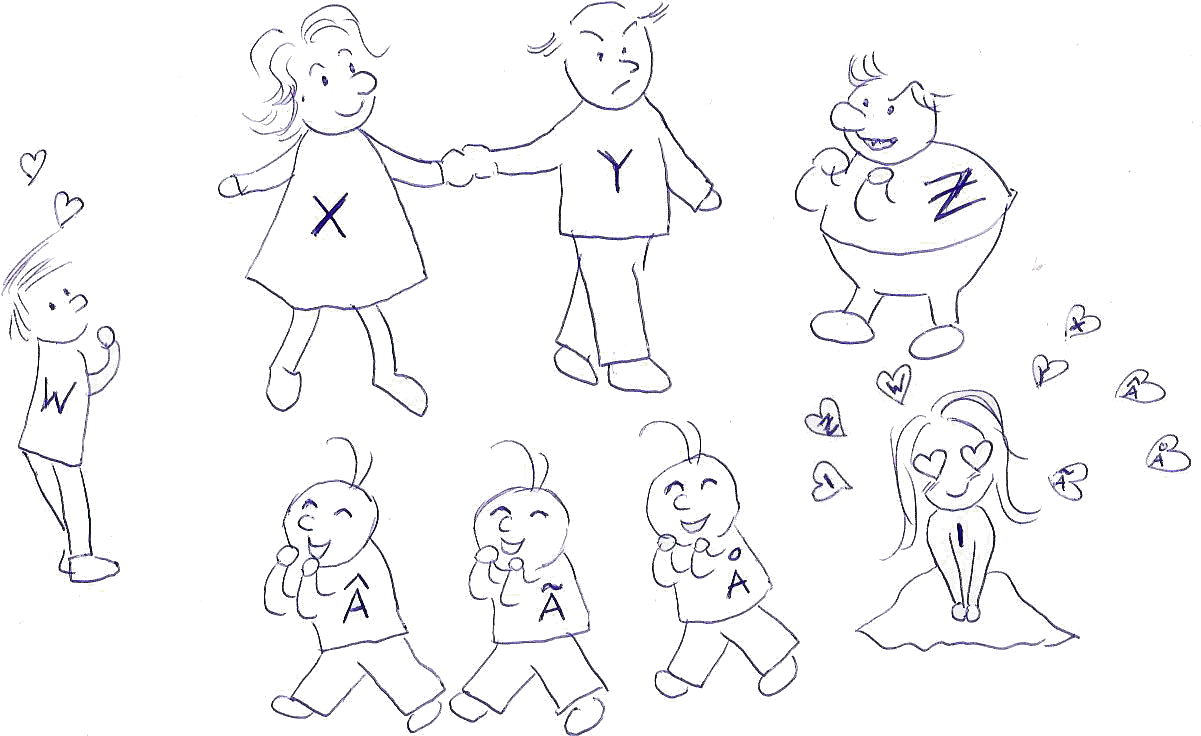
\includegraphics[scale=0.3]{relationen.png}
  \end{center}
}

\subsection[Initiale u. terminale Obj.]{Initiale und terminale Objekte}
\frame[t]{\frametitle{Initiale und terminale Objekte}
  \textbf{Definition:} Ein Objekt~$X$ einer Kategorie~$\C$ heißt genau dann
  \begin{itemize}
    \item \emph{initial}, wenn
      \[ \forall Y \in \Ob \C{:}\ \exists! f : X \to Y. \]
    \item \emph{terminal}, wenn
      \[ \forall Y \in \Ob \C{:}\ \exists! f : Y \to X. \]
  \end{itemize}

  \vfill
  \only<1>{\textbf{Frage:} Was ist ein terminales Objekt in~$\Set$?}
  \only<2>{%
    In $\Set$: \tabto{2.15cm} $\emptyset$ initial, $\{\star\}$ terminal.

    In $\R{-}\Vect$: \tabto{2.15cm} $\R^0$ initial und terminal.}
}

\subsection[Monos und Epis]{Mono- und Epimorphismen}
\frame[t]{\frametitle{Mono- und Epimorphismen}
  \textbf{Definition:}
  Ein Morphismus $f:X \to Y$ einer Kategorie~$\C$ heißt genau dann
  \begin{itemize}
    \item \emph{Monomorphismus}, \tabto{3.35cm}wenn für alle Objekte~$A \in \Ob \C$ \\
    \tabto{3.35cm}und $p,q:A \to X$ gilt:
    \[ f \circ p = f \circ q \quad\Longrightarrow\quad p = q. \]
    \item \emph{Epimorphismus}, \tabto{3.35cm}wenn für alle Objekte~$A \in \Ob \C$ \\
    \tabto{3.35cm}und $p,q:Y \to A$ gilt:
    \[ p \circ f = q \circ f \quad\Longrightarrow\quad p = q. \]
  \end{itemize}

  \textbf{Beobachtung} in $\Set$, $\Grp$ und $\R{-}\Vect$:
  \begin{align*}
    \text{$f$ Mono} &\Longleftrightarrow \text{$f$ injektiv.} \\
    \text{$f$ Epi} &\Longleftrightarrow \text{$f$ surjektiv.}
  \end{align*}
}

\subsection[Duale Kat.]{Die duale Kategorie einer Kategorie}
\frame[t]{\frametitle{Duale Kategorie}%
  \begin{itemize}
    \item \textbf{Definition:} Zu jeder Kategorie~$\C$ gibt es eine zugehörige
    \emph{duale Kategorie} $\C^\op$:
    \begin{align*}
      \Ob \C^\op &:= \Ob \C \\
      \Hom_{\C^\op}(X,Y) &:= \Hom_\C(Y,X)
    \end{align*}
    \item \textbf{Beispiel:} $\quad$ $X$ in $\C^\op$ initial
    $\quad\Longleftrightarrow\quad$ $X$ in $\C$ terminal
    \item \textbf{Beispiel:} $\quad$ $f$ in $\C^\op$ Mono $\quad\Longleftrightarrow\quad$ $f$ in $\C$ Epi
    \item \textbf{Nichttriviale Frage:} Wie kann man in konkreten
    Fällen~$\C^\op$ explizit (inhaltlich) beschreiben?
  \end{itemize}

  \begin{center}
    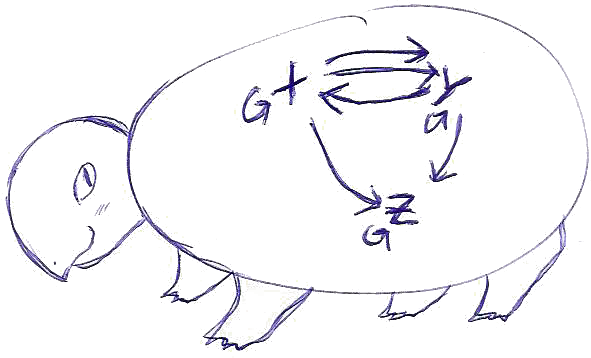
\includegraphics[scale=0.3]{kategorie.png}\quad
    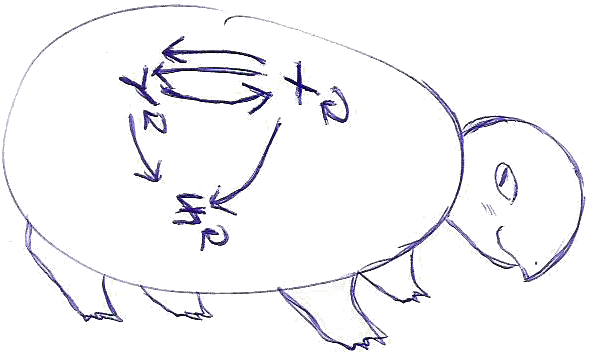
\includegraphics[scale=0.3]{kategorie-dual.png}
  \end{center}
}

\section{Anwendungen}
\frame[t]{\frametitle{Anwendungen}%
  \begin{itemize}
    \item Kategorientheorie liefert einen Leitfaden, \\ um richtige Definitionen
    zu formulieren.

    \item Triviales wird \emph{trivialerweise} trivial: \\
    \hil{Allgemeiner abstrakter Nonsens.}

    \item Konzeptionelle Vereinheitlichung: Viele Konstruktionen in der
    Mathematik sind Spezialfälle von allgemeinen kategoriellen: \\
    \hil{Limiten, Kolimiten, adjungierte Funktoren}

    \item Forschungsprogramm der Kategorifizierung,
          um tiefere Gründe für Altbekanntes zu finden.
  \end{itemize}

  \begin{tikzpicture}[remember picture,overlay]
    \node [xshift=-1cm,yshift=-3cm] at (current page.north east)
      {
\includegraphics[scale=0.3]{nonsens.png}};
  \end{tikzpicture}%
}

\end{document}
